\documentclass[crop,tikz]{standalone}
\usepackage{pgfplots}

\usetikzlibrary{arrows.meta}

% Vector field of a homogeneously electrically charged and rotating
% sphere shell of Radius R. In spherical coordinates, the magnetic
% field outside the sphere is
%
% \vec{B}(r,\theta,\varphi)
%   = \mu_0 m/(4\pi r^3)[3\vec{e}_r(\vec{e}_z\cdot\vec{e}_r) - \vec{e}_z]
%   = \mu_0 m/(4\pi r^3)[2\cos(\theta)\vec{e}_r + \sin(\theta)\vec{e}_\theta],
%
% where m = q\omega R^2/3 is the magnetic moment, q is the total
% charge of the sphere, \omega is the angular frequency of the
% rotation and \theta\in[0;\pi] and \varphi\in[0;2\pi). In cartesian
% coordinates one has
%
% \vec{B}(x,y,z)
%   = \mu_0 m/(4\pi r^5)[3xz\vec{e}_x + 3yz\vec{e}_y + (2z^2 - x^2 - y^2)\vec{e}_z].
%
% Inside the sphere the field is homogeneous.

\pgfplotsset{
  compat=1.18,
  inverted/.style = {
    every axis legend/.append style={
      draw=white,
      fill=hardblack,
      text=white
    }
  },
}

\begin{document}
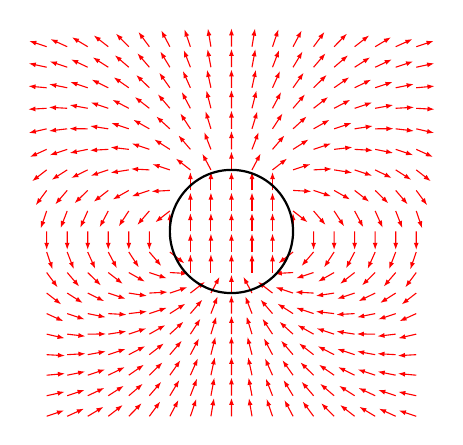
\begin{tikzpicture}
  \pgfmathsetmacro{\R}{1.0}; % radius of sphere
  \pgfmathsetmacro{\eps}{1.0e-9};
  \begin{axis}[
    width={0.6\linewidth},
    axis equal image,
    axis lines=middle,
    hide axis,
    view={0}{90},
    xmin=-3, xmax=3,
    ymin=-3, ymax=3,
    declare function = {
      rsq(\x,\z) = \x*\x + \z*\z;
      rabs(\x,\z) = sqrt(rsq(\x,\z));
      % magnetic field (inside and outside the sphere) for y=0 and \mu_0 m/(4\pi) = 1
      Bxraw(\x,\z) = (rabs(\x,\z) < \R) ? 0 : (3*\x*\z/rabs(\x,\z)^5);
      Bzraw(\x,\z) = (rabs(\x,\z) < \R) ? 1 : ((2*\z*\z - \x*\x)/rabs(\x,\z)^5);
      Bnorm(\x,\z) = sqrt(Bxraw(\x,\z)^2 + Bzraw(\x,\z)^2);
      % normalized magnetic field
      Bx(\x,\z) = (Bnorm(\x,\z) < \eps) ? (0/0) : (Bxraw(\x,\z)/Bnorm(\x,\z));
      Bz(\x,\z) = (Bnorm(\x,\z) < \eps) ? (0/0) : (Bzraw(\x,\z)/Bnorm(\x,\z));
    },
    clip=false,
    ]
    \addplot3[
      quiver={
        u={Bx(x,y)},
        v={Bz(x,y)},
        scale arrows=0.3,
      },
      -{Latex[length=1pt 4,width=1pt 2]},
      red,
      domain=-3:3, y domain=-3:3,
      samples=19, samples y=19,
    ] {0};
    % sphere
    \addplot[black, thick, domain=0:360, samples=240] ({\R*cos(x)},{\R*sin(x)});
  \end{axis}
\end{tikzpicture}
\end{document}
